\documentclass[11pt]{article}
\usepackage{listings}
\usepackage{tikz}
\usepackage{alltt}
\usepackage{hyperref}
\usepackage{url}
%\usepackage{algorithm2e}
\usetikzlibrary{arrows,automata,shapes}
\tikzstyle{block} = [rectangle, draw, fill=blue!20, 
    text width=5em, text centered, rounded corners, minimum height=2em]
\tikzstyle{bt} = [rectangle, draw, fill=blue!20, 
    text width=1em, text centered, rounded corners, minimum height=2em]

\newtheorem{defn}{Definition}
\newtheorem{crit}{Criterion}
\newcommand{\true}{\mbox{\sf true}}
\newcommand{\false}{\mbox{\sf false}}

\newcommand{\handout}[5]{
  \noindent
  \begin{center}
  \framebox{
    \vbox{
      \hbox to 5.78in { {\bf Software Testing, Quality Assurance and Maintenance } \hfill #2 }
      \vspace{4mm}
      \hbox to 5.78in { {\Large \hfill #5  \hfill} }
      \vspace{2mm}
      \hbox to 5.78in { {\em #3 \hfill #4} }
    }
  }
  \end{center}
  \vspace*{4mm}
}

\newcommand{\lecture}[4]{\handout{#1}{#2}{#3}{#4}{Lecture #1}}
\topmargin 0pt
\advance \topmargin by -\headheight
\advance \topmargin by -\headsep
\textheight 8.9in
\oddsidemargin 0pt
\evensidemargin \oddsidemargin
\marginparwidth 0.5in
\textwidth 6.5in

\parindent 0in
\parskip 1.5ex
%\renewcommand{\baselinestretch}{1.25}

%\renewcommand{\baselinestretch}{1.25}
% http://gurmeet.net/2008/09/20/latex-tips-n-tricks-for-conference-papers/
\newcommand{\squishlist}{
 \begin{list}{$\bullet$}
  { \setlength{\itemsep}{0pt}
     \setlength{\parsep}{3pt}
     \setlength{\topsep}{3pt}
     \setlength{\partopsep}{0pt}
     \setlength{\leftmargin}{1.5em}
     \setlength{\labelwidth}{1em}
     \setlength{\labelsep}{0.5em} } }
\newcommand{\squishlisttwo}{
 \begin{list}{$\bullet$}
  { \setlength{\itemsep}{0pt}
     \setlength{\parsep}{0pt}
    \setlength{\topsep}{0pt}
    \setlength{\partopsep}{0pt}
    \setlength{\leftmargin}{2em}
    \setlength{\labelwidth}{1.5em}
    \setlength{\labelsep}{0.5em} } }
\newcommand{\squishend}{
  \end{list}  }
\begin{document}

\lecture{22 --- March 2, 2015}{Winter 2015}{Patrick Lam}{version 1}

\section*{Graph Coverage for Specifications}
We'll move further up the abstraction chain now and talk about
testing based on specifications. Specification-based testing can
help ensure that a system doesn't drift too far from its intended 
behaviour, and tends to focus on higher-level concerns than 
the testing we've seen so far, which is based on properties of the source code.

\subsection*{Sequencing Constraints}
Libraries often come with constraints on permissible actions; we call
these constraints sequencing constraints.

\paragraph{Java Iterators.} {\sf Here are two possible constraints.}\\[2em]
 (1) A good practice is to always call
 {\tt hasNext()} before calling {\tt next()}. 
 (2) The Java API
 states that clients must not use an {\tt Iterator} after they
 have modified the underlying {\tt Collection}. For instance,
 {\tt c = new LinkedList(); c.add(o1); i = c.iterator(); i.next(); c.add(o2);
 i.next(); /* bad! */}

The general format of sequencing constraints is ``do X before Y'', or
``don't do W before A''. Here is another sequencing constraint, this
one implicit.

\begin{verbatim}
    /* @requires size() > 0 */
    public int dequeue() { ... }

    /* @ensures size() = \old(size()) + 1 */
    public void enqueue (int x) { ... }
\end{verbatim}

Assuming that the only way to increase {\tt size()} is by calling 
{\tt enqueue()}, then a client had better call {\tt enqueue()} before
calling {\tt dequeue()}.

It's generally useful to look for such constraints in code that
you're developing or testing, even if it's hard to identify them.
These constraints specify partial program properties. 

\paragraph{Using Sequencing Constraints.} Our approach will be to 
verify that sequencing constraints hold (or are never violated) on all
paths through a graph modelling the system under test.

\newpage
Let's consider the following three methods: 
\begin{itemize}
\item {\tt open(String fname)}
\item {\tt close()}
\item {\tt write(String line)}
\end{itemize}
and the following rules:
\begin{enumerate}
\item {\tt open(fn)} must be executed before any call to {\tt write(t)};
\item {\tt open(fn)} must be executed before any call to {\tt close()};
\item {\tt write(t)} must not execute after {\tt close()} unless {\tt open(fn)} has executed in between;
\item {\tt write(t)} should be executed before every {\tt close()};
\item {\tt close()} must not execute after {\tt close()} unless {\tt open(fn)} executes in between;
\item {\tt open(fn)} must not execute after {\tt open(fn)} unless {\tt close()} executes in between.
\end{enumerate}

{\sf How does this simplify reality?}

We will check these sequencing constraints on graphs, typically CFGs.

\begin{figure}[h]
\begin{center}
\begin{minipage}{.4\textwidth}
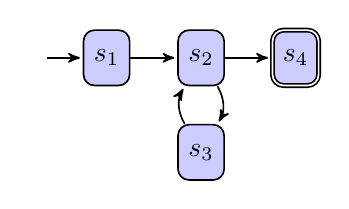
\begin{tikzpicture}[->,>=stealth',shorten >=1pt,auto,node distance=1.2cm,
                    semithick,initial text=]
  \node[initial,bt]   (s1)                     {$s_1$};
  \node[bt]           (s2) [right of=s1] {$s_2$};
  \node[bt]           (s3) [below of=s2] {$s_3$};
  \node[bt,accepting] (s4) [right of=s2] {$s_4$};

  \path (s1) edge node {} (s2)
        (s2) edge [bend left]  node {} (s3)
        (s3) edge [bend left] node {} (s2)
        (s2) edge node {} (s4);
\end{tikzpicture}
\caption{\label{fig:a} Simple Control-Flow Graph}
\end{minipage}~~~\
\begin{minipage}{.5\textwidth}
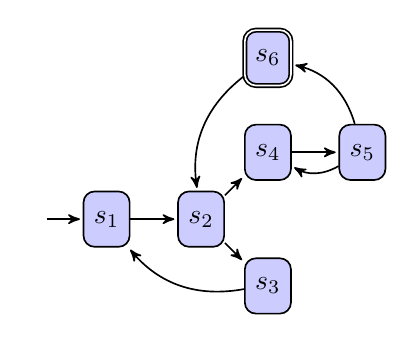
\begin{tikzpicture}[->,>=stealth',shorten >=1pt,auto,node distance=1.2cm,
                    semithick,initial text=]
  \node[initial,bt]   (s1)                     {$s_1$};
  \node[bt]           (s2) [right of=s1] {$s_2$};
  \node[bt]           (s3) [below right of=s2] {$s_3$};
  \node[bt]           (s4) [above right of=s2] {$s_4$};
  \node[bt]           (s5) [right of=s4] {$s_5$};
  \node[bt,accepting] (s6) [above of=s4] {$s_6$};

  \path (s1) edge node {} (s2)
        (s2) edge node {} (s3)
             edge node {} (s4)
        (s3) edge [bend left] node {} (s1)
        (s4) edge node {} (s5)
        (s5) edge [bend left] node {} (s4)
             edge [bend right] node {} (s6)
        (s6) edge [bend right] node {} (s2);
\end{tikzpicture}
\caption{\label{fig:b} More Complicated Control-Flow Graph}
\end{minipage}

\end{center}
\end{figure}

\paragraph{Static approach.} We can deduce, without running anything 
(i.e. statically), that the
program in Figure~\ref{fig:a} must satisfy all of the properties
except for the one which requires that {\tt write} occur before {\tt
  close}. The model of the program in Figure~\ref{fig:b} shows that it
may violate the property that requires no writes to occur after
closes. However, the back edge $(s_5, s_4)$ might be infeasible.

\paragraph{Dynamic approach.} By running the programs with suitable
test cases, we could explicitly identify violating cases. If we are
unable to find any violating cases, we can have some confidence that,
in practice, the program never violates the properties.

\subsection*{Test Requirements} We can use test requirements to verify 
sequencing constraints in two ways: (1) we can create tests that satisfy
various coverage criteria, thus suggesting that the program probably
doesn't violate properties; or (2) we can set up test requirements,
if satisfied, exhibit executions where constraints are violated.
We might,
for instance, set up the following test requirements:
\begin{itemize}
\item cover every path from the start to all {\tt write()} nodes that
don't go through any {\tt open()} nodes; 
\item cover every path from the start to all {\tt close()} nodes that
don't go through any {\tt open()} nodes;
\item etc.
\end{itemize}
We are hoping that such test requirements will be infeasible; any
program that meets the specification will be unable to satisfy these
test requirements.


\section*{Testing State Behaviour of Software via FSMs}

We can also model the behaviour of software using a finite-state
machine. Such models are higher-level than the control-flow graphs and
call graphs that we've seen to date. They instead capture the design
of the software. There is generally no obvious mapping between a
design-level FSM and the code.

We propose the use of graph coverage criteria to test with FSMs.
\begin{itemize}
\item nodes: software states (e.g. sets of values for key variables);
\item edges: transitions between software states, i.e. something changes
in the environment or someone enters a command.
\end{itemize}
The FSM enables exploration of the software system's state space.  A
software state consists of values for (possibly abstract) program
variables, while a transition represents a change to these program
variables. Often transitions are guarded by preconditions and
postconditions; the preconditions must hold for the FSM to take the
corresponding transition, and the postconditions are guaranteed to
hold after the FSM has taken the transition.

\begin{itemize}
\item node coverage: visiting every FSM state = stage coverage;
\item edge coverage: visiting every FSM transition = transition coverage;
\item edge-pair coverage: actually useful for FSMS; transition-pair, two-trip coverage.
\end{itemize}

Dataflow coverage doesn't apply very well to FSMs. We could associate
defs and uses with FSM edges; however, even if we make sure to achieve
edge coverage, we might not be able to individually control all of the
abstract variables underlying the FSM.

\paragraph{Exercise.}  Create a Finite State Machine for some system that
you're familiar with.
%(In class, we saw a traffic light (AM) and for baking 
%cookies (PM); with the baking cookies example, we saw both an imperative
%FSM which is CFG-like and a more state-based FSM. We had a question about
%whether we could split the state-based FSM into an oven FSM and an
%ingrediate FSM. Yes, we could, but then we'd have to understand how
%to synchronize different FSMs, which is beyond the scope of this class.)

\subsection*{Deriving Finite-State Machines}
You might have to test software which doesn't come with a handy FSM.
Deriving an FSM aids your understanding of the software. (You might
be finding yourself re-deriving the same FSM as the software evolves;
design information tends to become stale.)

We've seen iComment and Daikon for obtaining sequencing constraints from
comments/documentation and from the code.

%% Four techniques for deriving FSMs:
%% \begin{itemize}
%% \item use control-flow graphs;
%% \item use higher-level software structure;
%% \item model software's state variables; or
%% \item use specifications.
%% \end{itemize}

\paragraph{Control-Flow Graphs.} Does not really give FSMs.
\begin{itemize}
\item nodes aren't really states; they just abstract the program
counter;
\item inessential nondeterminism due e.g. to method calls;
\item can only build these when you have an implementation;
\item tend to be large and unwieldy.
\end{itemize}

\paragraph{Software Structure.} Better than CFGs.
\begin{itemize}
\item subjective (which is not necessarily bad);
\item requires lots of effort;
\item requires detailed design information and knowledge of system.
\end{itemize}

\paragraph{Modelling State.} 
This approach is more mechanical: once you've chosen relevant state
variables and abstracted them, you need not think much.

You can also remove impossible states from such an FSM, for instance
by using domain knowledge.

\paragraph{Specifications.}
These are similar to building FSMs based on software structure.
Generally cleaner and easier to understand. Should resemble UML
statecharts.

\paragraph{General Discussion.} Advantages of FSMs:
\begin{itemize}
\item enable creation of tests before implementation;
\item easier to analyze an FSM than the code.
\end{itemize}
Disadvantages:
\begin{itemize}
\item abstract models are not necessarily exhaustive;
\item subjective (so they could be poorly done);
\item FSM may not match the implementation.
\end{itemize}


\end{document}
